\documentclass[10pt,answers]{exam}
\usepackage[legalpaper,bindingoffset=0in,left=.6in,right=0.8in,top=0.4in,bottom=0.7in,headsep=.5\baselineskip]{geometry}
\usepackage[utf8]{inputenc}
\usepackage{graphicx}
\usepackage{listings}
\usepackage{enumitem}
\usepackage{amsmath}
\usepackage{multirow}
\usepackage{multicol}
\usepackage{caption}
\usepackage{tabularx}
\usepackage{url}
\usepackage{amssymb}
\usepackage{array}
\usepackage{tikz}
\usetikzlibrary{shapes.callouts, positioning, arrows.meta, shapes.geometric, shadows, calc, patterns, 3d, backgrounds, shadings, decorations.markings}
\usepackage{adjustbox}
\usepackage{ragged2e}
\usepackage{pgfplots}
\pgfplotsset{compat=1.18} % Added to suppress pgfplots warning

\def\changemargin#1#2{\list{}{\rightmargin#2\leftmargin#1}\item[]}
\let\endchangemargin=\endlist 

\usepackage{xcolor}
\definecolor{mGreen}{rgb}{0,0.6,0}
\definecolor{mGray}{rgb}{0.5,0.5,0.5}
\definecolor{mPurple}{rgb}{0.58,0,0.82}
\definecolor{backgroundColour}{rgb}{0.95,0.95,0.92}
\lstset{
    language=C,
    basicstyle=\ttfamily\small,
    aboveskip={1.0\baselineskip},
    belowskip={1.0\baselineskip},
    columns=fixed,
    extendedchars=true,
    breaklines=true,
    tabsize=4,
    prebreak=\raisebox{0ex}[0ex][0ex]{\ensuremath{\hookleftarrow}},
    frame=lines,
    showtabs=false,
    showspaces=false,
    showstringspaces=false,
    keywordstyle=\color[rgb]{0.627,0.126,0.941},
    commentstyle=\color[rgb]{0.133,0.545,0.133},
    stringstyle=\color[rgb]{01,0,0},
    numbers=left,
    numberstyle=\small,
    stepnumber=1,
    numbersep=10pt,
    captionpos=t,
    escapeinside={\%*}{*)}
}

\pointsdroppedatright

\title{
\vspace{-1.5cm} % Pull the title up closer to the top margin
\begin{changemargin}{0.68cm}{0.68cm} 
\normalsize Class Test 4 Solutions\hfill {July 2025}\\
\end{changemargin} 
\vspace{.4cm}
\large BANGLADESH UNIVERSITY OF ENGINEERING AND TECHNOLOGY\\
\vspace{.1cm}
Department of Computer Science and Engineering\\
\vspace{.2cm}
Course Code: CSE 219 \hspace{.1cm} Course Title: Signals and Linear Systems\\
\vspace{.2cm}
\textbf{Time: 25 minutes} \hspace{2.2cm} \textbf{Marks: 20}
\begin{changemargin}{0.68cm}{0.68cm} 
\normalsize Student Name: \underline{Md. Ashrafur Rahman Khan} \hfill Student ID: \underline{1905005}\\
\end{changemargin} 
}
\date{} % Prevents today's date from rendering below the title

\begin{document}

\maketitle
\thispagestyle{empty} % Removes the page number from the first page
\vspace{-2.4cm} % Reduces the default space left by maketitle 

\begin{center}
    Answer \textbf{exactly 2 out of Questions 1--4}. \textbf{Question 5 is mandatory.} Answer concisely.
\end{center}

\begin{questions}

    % Question 1
    \question Consider the signal $x[n]$ defined as follows for $N=4$: \hfill [8]
    \[
        x[n] = \begin{cases} 1, & \text{if } n=0 \\ 0, & \text{if } 1 \leq n < N \end{cases}
    \]

    \begin{parts}
        \part Compute the 4-point radix-2 DIT FFT of the signal. Draw a butterfly diagram and show your calculations on the diagram.
        \begin{solution}
            The sequence is $x[n] = \{1, 0, 0, 0\}$.
            For the 4-point radix-2 DIT FFT, the inputs are arranged in bit-reversed order: $x[0], x[2], x[1], x[3]$, which corresponds to $1, 0, 0, 0$.

            \begin{center}
                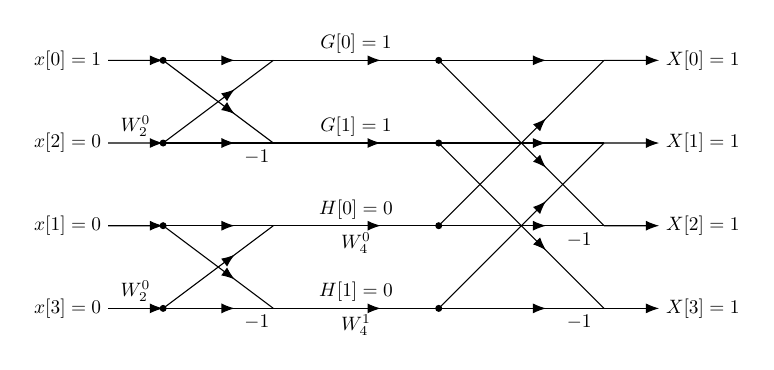
\begin{tikzpicture}[>=Latex, scale=0.7, transform shape,
                        mid arrow/.style={postaction={decorate,decoration={markings, mark=at position 0.65 with {\arrow{Latex}}}}}]
                    % Inputs
                    \node[left] (x0) at (0, 4.5) {$x[0]=1$};
                    \node[left] (x2) at (0, 3.0) {$x[2]=0$};
                    \node[left] (x1) at (0, 1.5) {$x[1]=0$};
                    \node[left] (x3) at (0, 0.0) {$x[3]=0$};

                    % Outputs
                    \node[right] (X0) at (10, 4.5) {$X[0]=1$};
                    \node[right] (X1) at (10, 3.0) {$X[1]=1$};
                    \node[right] (X2) at (10, 1.5) {$X[2]=1$};
                    \node[right] (X3) at (10, 0.0) {$X[3]=1$};

                    % Stage 1 Nodes
                    \coordinate (s1a0) at (1, 4.5); \coordinate (s1b0) at (3, 4.5); \coordinate (s1c0) at (4, 4.5);
                    \coordinate (s1a1) at (1, 3.0); \coordinate (s1b1) at (3, 3.0); \coordinate (s1c1) at (4, 3.0);
                    \coordinate (s1a2) at (1, 1.5); \coordinate (s1b2) at (3, 1.5); \coordinate (s1c2) at (4, 1.5);
                    \coordinate (s1a3) at (1, 0.0); \coordinate (s1b3) at (3, 0.0); \coordinate (s1c3) at (4, 0.0);

                    % Stage 2 Nodes
                    \coordinate (s2a0) at (6, 4.5); \coordinate (s2b0) at (9, 4.5);
                    \coordinate (s2a1) at (6, 3.0); \coordinate (s2b1) at (9, 3.0);
                    \coordinate (s2a2) at (6, 1.5); \coordinate (s2b2) at (9, 1.5);
                    \coordinate (s2a3) at (6, 0.0); \coordinate (s2b3) at (9, 0.0);

                    % Draw horizontal background lines implicitly through segments

                    % Incoming to Stage 1
                    \draw[->] (x0) -- (s1a0);
                    \draw[->] (x2) -- node[above] {$W_2^0$} (s1a1);
                    \draw[->] (x1) -- (s1a2);
                    \draw[->] (x3) -- node[above] {$W_2^0$} (s1a3);

                    % Stage 1 crossovers
                    \filldraw (s1a0) circle(1.5pt) (s1a1) circle(1.5pt) (s1a2) circle(1.5pt) (s1a3) circle(1.5pt);
                    \draw[mid arrow] (s1a0) -- (s1b0);
                    \draw[mid arrow] (s1a1) -- (s1b0);
                    \draw[mid arrow] (s1a0) -- (s1b1);
                    \draw[mid arrow] (s1a1) -- node[below, pos=0.85] {$-1$} (s1b1);

                    \draw[mid arrow] (s1a2) -- (s1b2);
                    \draw[mid arrow] (s1a3) -- (s1b2);
                    \draw[mid arrow] (s1a2) -- (s1b3);
                    \draw[mid arrow] (s1a3) -- node[below, pos=0.85] {$-1$} (s1b3);

                    % Intermediate G and H values
                    \draw[mid arrow] (s1b0) -- node[above] {$G[0]=1$} (s2a0);
                    \draw[mid arrow] (s1b1) -- node[above] {$G[1]=1$} (s2a1);
                    \draw[mid arrow] (s1b2) -- node[above] {$H[0]=0$} node[below] {$W_4^0$} (s2a2);
                    \draw[mid arrow] (s1b3) -- node[above] {$H[1]=0$} node[below] {$W_4^1$} (s2a3);

                    % Stage 2 crossovers
                    \filldraw (s2a0) circle(1.5pt) (s2a1) circle(1.5pt) (s2a2) circle(1.5pt) (s2a3) circle(1.5pt);
                    \draw[mid arrow] (s2a0) -- (s2b0);
                    \draw[mid arrow] (s2a2) -- (s2b0);
                    \draw[mid arrow] (s2a1) -- (s2b1);
                    \draw[mid arrow] (s2a3) -- (s2b1);

                    \draw[mid arrow] (s2a0) -- (s2b2);
                    \draw[mid arrow] (s2a2) -- node[below, pos=0.85] {$-1$} (s2b2);
                    \draw[mid arrow] (s2a1) -- (s2b3);
                    \draw[mid arrow] (s2a3) -- node[below, pos=0.85] {$-1$} (s2b3);

                    % Final to outputs
                    \draw[->] (s2b0) -- (X0);
                    \draw[->] (s2b1) -- (X1);
                    \draw[->] (s2b2) -- (X2);
                    \draw[->] (s2b3) -- (X3);

                \end{tikzpicture}
            \end{center}
        \end{solution}
        \part If $x[n]$ is viewed as samples of an aperiodic continuous-time signal, what might be a continuous-time signal corresponding to it?
        \begin{solution}
            A continuous-time signal corresponding to it could be the Dirac delta function $\delta(t)$ or a very narrow pulse at $t=0$, since the sequence only has a single non-zero value at $n=0$.
        \end{solution}
        \part Based on your answer in (b), interpret your result from (a). If the sequence is zero-padded to length $32$, what is its 32-point DFT? Briefly justify.
        \begin{solution}
            The continuous-time Fourier transform of $\delta(t)$ is $1$ for all frequencies. Similarly, the DTFT of the single impulse $\delta[n]$ is $X(e^{j\omega}) = 1$ for all $\omega$. The $N$-point DFT evaluates $X(e^{j\omega})$ exactly at evenly spaced discrete frequencies. Thus, it is simply $N$ equispaced samples of the continuous DTFT exactly over one $2\pi$ period. This gives $X[k] = 1$ for all $k$, which matches our result from (a).

            By zero-padding the sequence to a total length $M=32$, taking the $32$-point DFT samples the \textit{same} continuous DTFT spectrum $X(e^{j\omega})$, but at a much finer resolution of $2\pi/32$. Since the underlying DTFT is constantly $1$, the 32-point DFT $X_{32}[k]$ will just be $1$ for all $k = 0, \dots, 31$.
        \end{solution}
        \part In a radix-2 DIT FFT, we typically use bit-reversed order for the input $x[n]$. Imagine you forgot to use bit-reversed order and used natural order for the input instead, resulting in a sequence $X'[k]$. Determine the signal $x'[n]$ whose DFT is actually $X'[k]$.
        \begin{solution}
            The FFT algorithm expects the input at algorithmic index $n$ to be $x[r(n)]$, where $r(n)$ is the bit-reversed value of $n$. So if we provide $x[n]$ directly, the algorithm mathematically processes it as if it were the bit-reversed version of some actual virtual signal $x'[n]$. Thus,  $x'[n] = x[r(n)]$. The signal $x'[n]$ is simply the bit-reversed sequence of $x[n]$.

            In this specific case, $x[n] = \{1, 0, 0, 0\}$ for $n=0, 1, 2, 3$. The bit-reversed indices process as follows:
            $x'[0] = x[0] = 1$,
            $x'[1] = x[2] = 0$,
            $x'[2] = x[1] = 0$,
            $x'[3] = x[3] = 0$.
            Thus, $x'[n] = \{1, 0, 0, 0\}$. Since the only non-zero position is at index 0 and remains unchanged, $x'[n] = x[n]$.
        \end{solution}
    \end{parts}
    \vspace{0.2cm}

    % Question 2
    \question In many cases, the radix-4 FFT is highly efficient. Suppose you are deriving the radix-4 DIT Cooley-Tukey algorithm. You have already established that for $0 \leq k < N/4$: \hfill [8]
    \[
        X[k] = G_0[k] + W_N^k G_1[k] + W_N^{2k} G_2[k] + W_N^{3k} G_3[k]
    \]
    Where \[
        G_m[k] = \sum_{r=0}^{N/4-1} x[4r+m]\, W_{N/4}^{kr}, \qquad m=0,1,2,3
    \].

    \begin{parts}
        \part Derive the formulas for $X[k+N/4]$, $X[k+2N/4]$, and $X[k+3N/4]$.
        \begin{solution}
            Since $G_m[k]$ is a DFT of length $N/4$, it is periodic with period $N/4$, so $G_m[k + pN/4] = G_m[k]$.
            Also, note the twiddle factor phase shifts: $W_N^{pN/4} = e^{-j \frac{2\pi}{N} \frac{pN}{4}} = e^{-j \frac{\pi}{2} p} = (-j)^p$.
            Using these properties:
            \begin{align*}
                X[k+N/4]  & = G_0[k] + W_N^{k+N/4} G_1[k] + W_N^{2(k+N/4)} G_2[k] + W_N^{3(k+N/4)} G_3[k]    \\
                          & = G_0[k] - j W_N^k G_1[k] - W_N^{2k} G_2[k] + j W_N^{3k} G_3[k]                  \\
                X[k+2N/4] & = G_0[k] + W_N^{k+2N/4} G_1[k] + W_N^{2(k+2N/4)} G_2[k] + W_N^{3(k+2N/4)} G_3[k] \\
                          & = G_0[k] - W_N^k G_1[k] + W_N^{2k} G_2[k] - W_N^{3k} G_3[k]                      \\
                X[k+3N/4] & = G_0[k] + W_N^{k+3N/4} G_1[k] + W_N^{2(k+3N/4)} G_2[k] + W_N^{3(k+3N/4)} G_3[k] \\
                          & = G_0[k] + j W_N^k G_1[k] - W_N^{2k} G_2[k] - j W_N^{3k} G_3[k]
            \end{align*}
        \end{solution}
        \part Draw the radix-4 butterfly for the case $N=4$. \\
        \textit{Hint: Instead of just $\pm 1$, there will also be multiplications involving $\pm j$.}
        \begin{solution}
            For $N=4$, $N/4 = 1$, so $G_m[0] = x[m]$. There is only $k=0$ to evaluate for each branch. The equations simplify to:
            \begin{align*}
                X[0] & = x[0] + x[1] + x[2] + x[3]   \\
                X[1] & = x[0] - jx[1] - x[2] + jx[3] \\
                X[2] & = x[0] - x[1] + x[2] - x[3]   \\
                X[3] & = x[0] + jx[1] - x[2] - jx[3]
            \end{align*}

            \begin{center}
                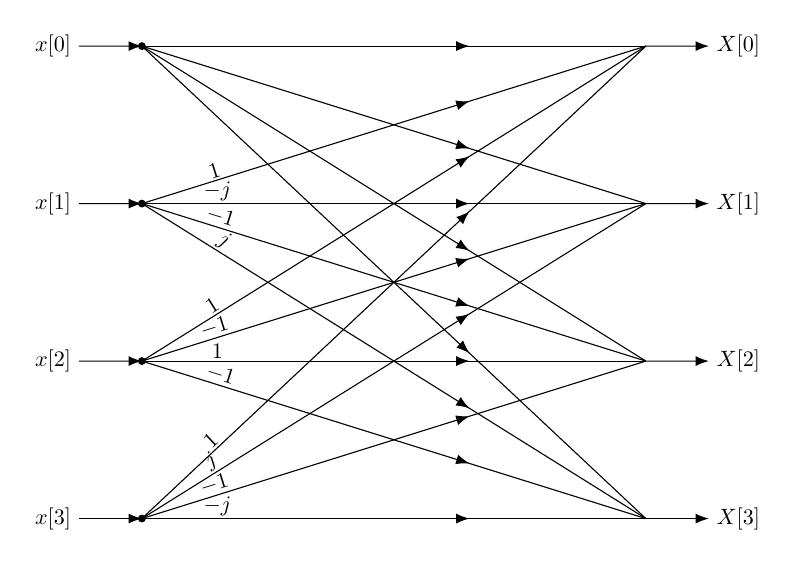
\begin{tikzpicture}[>=Latex, scale=0.8, transform shape,
                        mid arrow/.style={postaction={decorate,decoration={markings, mark=at position 0.65 with {\arrow{Latex}}}}}]
                    % Inputs
                    \node[left] (x0) at (0, 7.5) {$x[0]$};
                    \node[left] (x1) at (0, 5.0) {$x[1]$};
                    \node[left] (x2) at (0, 2.5) {$x[2]$};
                    \node[left] (x3) at (0, 0.0) {$x[3]$};

                    % Outputs
                    \node[right] (X0) at (10, 7.5) {$X[0]$};
                    \node[right] (X1) at (10, 5.0) {$X[1]$};
                    \node[right] (X2) at (10, 2.5) {$X[2]$};
                    \node[right] (X3) at (10, 0.0) {$X[3]$};

                    \coordinate (in0) at (1, 7.5); \coordinate (out0) at (9, 7.5);
                    \coordinate (in1) at (1, 5.0); \coordinate (out1) at (9, 5.0);
                    \coordinate (in2) at (1, 2.5); \coordinate (out2) at (9, 2.5);
                    \coordinate (in3) at (1, 0.0); \coordinate (out3) at (9, 0.0);

                    \filldraw (in0) circle(1.5pt) (in1) circle(1.5pt) (in2) circle(1.5pt) (in3) circle(1.5pt);

                    \draw[->] (x0) -- (in0); \draw[->] (x1) -- (in1);
                    \draw[->] (x2) -- (in2); \draw[->] (x3) -- (in3);

                    \draw[->] (out0) -- (X0); \draw[->] (out1) -- (X1);
                    \draw[->] (out2) -- (X2); \draw[->] (out3) -- (X3);

                    % Lines showing components
                    % from in0
                    \draw[mid arrow] (in0) -- (out0);
                    \draw[mid arrow] (in0) -- (out1);
                    \draw[mid arrow] (in0) -- (out2);
                    \draw[mid arrow] (in0) -- (out3);

                    % from in1
                    \draw[mid arrow] (in1) -- node[pos=0.15, above, sloped, inner sep=1pt] {$1$} (out0);
                    \draw[mid arrow] (in1) -- node[pos=0.15, above, sloped, inner sep=1pt] {$-j$} (out1);
                    \draw[mid arrow] (in1) -- node[pos=0.15, above, sloped, inner sep=1pt] {$-1$} (out2);
                    \draw[mid arrow] (in1) -- node[pos=0.15, above, sloped, inner sep=1pt] {$j$} (out3);

                    % from in2
                    \draw[mid arrow] (in2) -- node[pos=0.15, above, sloped, inner sep=1pt] {$1$} (out0);
                    \draw[mid arrow] (in2) -- node[pos=0.15, above, sloped, inner sep=1pt] {$-1$} (out1);
                    \draw[mid arrow] (in2) -- node[pos=0.15, above, sloped, inner sep=1pt] {$1$} (out2);
                    \draw[mid arrow] (in2) -- node[pos=0.15, above, sloped, inner sep=1pt] {$-1$} (out3);

                    % from in3
                    \draw[mid arrow] (in3) -- node[pos=0.15, above, sloped, inner sep=1pt] {$1$} (out0);
                    \draw[mid arrow] (in3) -- node[pos=0.15, above, sloped, inner sep=1pt] {$j$} (out1);
                    \draw[mid arrow] (in3) -- node[pos=0.15, above, sloped, inner sep=1pt] {$-1$} (out2);
                    \draw[mid arrow] (in3) -- node[pos=0.15, above, sloped, inner sep=1pt] {$-j$} (out3);

                \end{tikzpicture}
            \end{center}
        \end{solution}
    \end{parts}
    \vspace{0.2cm}

    % Question 3
    \question Consider two polynomials: \hfill [8]
    \[
        A(x) = \sum_{n=0}^{N-1} a[n] x^n \quad \text{and} \quad B(x) = \sum_{n=0}^{N-1} b[n] x^n
    \]
    You want to compute their product, $C(x) = A(x)B(x)$.

    \begin{parts}
        \part Provide a simple, naive algorithm to find the polynomial $C(x)$ and analyze its time complexity.
        \begin{solution}
            A naive algorithm expands the product algebraically.
            \begin{lstlisting}
function NaivePolynomialMult(a, b, N):
    // a and b are arrays of size N
    c = array of size 2N-1 initialized to 0
    for i from 0 to N-1:
        for j from 0 to N-1:
            c[i + j] = c[i + j] + a[i] * b[j]
    return c
\end{lstlisting}
            Because there are two nested loops of size $N$, the time complexity is $O(N^2)$.
        \end{solution}
        \part If we express $C(x)$ as the sum $\sum c[n]x^n$, determine the valid range for $n$ and provide a general formula for the coefficients $c[n]$.
        \begin{solution}
            The maximum degree in $C(x)$ is $(N-1) + (N-1) = 2N-2$. The minimum degree is $0$. Therefore, the valid range for $n$ is $0 \leq n \leq 2N-2$.

            First, the standard convolution sum is $c[n] = \sum_{k=0}^{N-1} a[k]b[n-k]$, assuming $a$ and $b$ are implicitly zero-padded outside the range $[0, N-1]$.

            To find the exact non-zero bounds for a specific $n$: we know $a[k]$ is defined for $0 \le k \le N-1$. Similarly, $b[n-k]$ is defined for $0 \le n-k \le N-1$.
            From $n-k \ge 0$, we get $k \le n$. Combining with $k \le N-1$ gives the upper bound: $k \le \min(n, N-1)$.
            From $n-k \le N-1$, we get $k \ge n-N+1$. Combining with $k \ge 0$ gives the lower bound: $k \ge \max(0, n-N+1)$.
            Applying these bounds results in the highly specific general formula:
            \[
                c[n] = \sum_{k=\max(0, n-N+1)}^{\min(n, N-1)} a[k]b[n-k]
            \]
        \end{solution}
        \part Express the coefficient sequence $c[n]$ as a convolution.
        \begin{solution}
            The coefficient sequence $c[n]$ is exactly the linear convolution of the sequences $a[n]$ and $b[n]$:
            \[
                c[n] = (a * b)[n] = \sum_{k=-\infty}^{\infty} a[k]b[n-k]
            \]
            where $a[n]$ and $b[n]$ are assumed to be zero outside the range $0 \leq n \leq N-1$.
        \end{solution}
        \part Propose a more efficient algorithm to compute $C(x)$ and analyze the time complexity of your proposed algorithm.
        \begin{solution}
            An efficient algorithm uses the Fast Fourier Transform (FFT) to perform fast linear convolution:
            \begin{lstlisting}
function FastPolynomialMult(a, b, N):
    // Find next power of 2 >= 2N - 1
    M = NextPowerOfTwo(2N - 1)
    // Zero-pad to length M
    a_padded = ZeroPad(a, M)
    b_padded = ZeroPad(b, M)
    // Transform to frequency domain
    A = FFT(a_padded)
    B = FFT(b_padded)
    // Pointwise multiplication
    for k from 0 to M-1:
        C[k] = A[k] * B[k]
    // Inverse transform
    c = IFFT(C)
    // Return the First 2N-1 coefficients
    return c[0 ... 2N-2]
\end{lstlisting}
            \textbf{Complexity:} The zero-padding takes $O(N)$ time. The two forward FFTs and one inverse FFT of length $M \approx 2N$ each take $O(M \log M) = O(N \log N)$ running time. The pointwise multiplication takes $O(M) = O(N)$ time. Overall time complexity is $O(N \log N)$, which is significantly faster than the naive $O(N^2)$ algorithm.
        \end{solution}
    \end{parts}
    \vspace{0.2cm}

    % Question 4
    \question In image processing, we often use a 2-dimensional version of the DFT, which is defined as: \hfill [8]
    \[
        X[k_1,k_2]
        =
        \sum_{n_1=0}^{N_1-1}\sum_{n_2=0}^{N_2-1}
        x[n_1,n_2]\,
        W_{N_1}^{k_1 n_1}
        W_{N_2}^{k_2 n_2}
    \]
    Where $x[n_1, n_2]$ is an $N_1 \times N_2$ matrix and $W_N^k = e^{-j2\pi k/N}$.

    \begin{parts}
        \part What is the time complexity of a naive algorithm used to compute the 2D DFT?
        \begin{solution}
            For each of the $N_1 N_2$ frequency pairs $(k_1, k_2)$, the naive algorithm evaluates a double sum involving $N_1 N_2$ terms:
            \begin{lstlisting}
function Naive2D_DFT(x, N1, N2):
    X = matrix of size N1 x N2 initialized to 0
    for k1 from 0 to N1-1:
        for k2 from 0 to N2-1:
            for n1 from 0 to N1-1:
                for n2 from 0 to N2-1:
                    X[k1, k2] += x[n1, n2]*exp(-j*2*pi*(k1*n1/N1 + k2*n2/N2))
    return X
\end{lstlisting}
            Thus, it takes $O(N_1 N_2)$ operations per frequency, leading to an overall time complexity of $O((N_1 N_2)^2) = O(N_1^2 N_2^2)$.
        \end{solution}
        \part How can you interpret the given formula as two successive 1D DFT operations?
        \begin{solution}
            We can separate the summations as follows:
            \[
                X[k_1,k_2] = \sum_{n_1=0}^{N_1-1} \underbrace{\left( \sum_{n_2=0}^{N_2-1} x[n_1,n_2]\, W_{N_2}^{k_2 n_2} \right)}_{\text{1D DFT along rows}} W_{N_1}^{k_1 n_1}
            \]
            The inner sum is simply a 1D DFT of length $N_2$ performed along each row $n_1$ of the matrix. Let this result be a temporary matrix $X'[n_1, k_2]$.
            Then, the outer sum computes a 1D DFT of length $N_1$ down each column $k_2$ of the temporary matrix $X'$.
        \end{solution}
        \part Propose an efficient algorithm (2D FFT) for computing this and analyze its complexity.
        \begin{solution}
            Using the interpretation from part (b), we can compute the 2D DFT efficiently by leveraging 1D FFT algorithms (known as the row-column algorithm):
            \begin{lstlisting}
function Fast2D_DFT(x, N1, N2):
    X_temp = matrix of size N1 x N2
    // 1D FFT along rows
    for n1 from 0 to N1-1:
        X_temp[n1, :] = FFT_1D(x[n1, :], N2) 
    X = matrix of size N1 x N2
    // 1D FFT down columns
    for k2 from 0 to N2-1:
        X[:, k2] = FFT_1D(X_temp[:, k2], N1)
    return X
\end{lstlisting}
            \textbf{Complexity Analysis:}
            The first step requires $N_1$ independent FFTs of length $N_2$, taking $O(N_1 \cdot N_2 \log N_2)$ total operations.
            The second step requires $N_2$ independent FFTs of length $N_1$, taking $O(N_2 \cdot N_1 \log N_1)$ total operations.
            Adding them together yields $O(N_1 N_2 \log N_2 + N_1 N_2 \log N_1) = O(N_1 N_2 \log(N_1 N_2))$. This is much faster than the naive $O(N_1^2 N_2^2)$.
        \end{solution}
        \part What is the primary difference between your 2D FFT algorithm and Bailey's FFT algorithm?
        \begin{solution}
            While both algorithms use row and column 1D FFTs on a 2D matrix structure, they solve fundamentally different problems. Bailey's FFT algorithm computes a \textbf{1D FFT} of length $N=N_1 N_2$ by mapping a 1D sequence into a 2D matrix. Critically, it requires intermediate multiplications by \textbf{twiddle factors} ($W_N^{n_1 k_2}$) after the row FFTs and before performing the column FFTs.
            The 2D FFT algorithm computes the \textbf{2D DFT} of a naturally 2D signal and involves \textbf{no internal twiddle factors} between the sequence of row and column FFTs.
        \end{solution}
    \end{parts}
    \vspace{0.2cm}

    % Question 5
    \question[4] Thank you for attending the classes and participating in this CT. \hfill [4]
    \begin{solution}
        You're welcome!
    \end{solution}

\end{questions}

\end{document}
